\chapter{Introduction}

\section{Motivation}

While there has been plenty of research into simulating sound propagation using both geometric and numerical methods,
nearly all of it only concerns itself with static scenes,
where neither objects within the scene nor the sound emitter nor receiver move with time.
\newline
Simulation of dynamic or moving scenes is mostly unexplored.
This is mostly because it is only really relevant for scenarios
where objects or receivers can move at speeds within one or two orders of magnitude from the ray's travelling speed;
If this condition is not fulfilled,
the error introduced from the snapshot method described below becomes minimal enough to be disregarded.
\newline
For light, the travelling wave relevant to computer graphics, this condition does not apply as
light famously travels at approximately \(3 \cdot 10^{8} m/s\).
As a reference, the fastest velocity achieved by humans is approximately \(1.1 \cdot 10^4 m/s\) during the launch of Apollo 10.
Seeing as even this extreme case is four orders of magnitude smaller than the speed of light,
errors introduced to computer graphics by the snapshot method are especially small.
\newline
Only a comparatively small part of the research into ray tracing comes from outside of computer graphics to begin with,
and even in other fields, such as acoustics simulation,
the error introduced by the snapshot method is only relevant in edge cases.
All of this makes simulation of moving scenes a rather niche problem.
\newline
Despite this, some research into simulating moving or dynamic scenes' acoustics has been done:
\newline
Raghuvanshi et al.~\cite{RS10} explore a numerical approach to handle dynamically moving emitters and receivers,
but do not look into moving objects within the scene.
\newline
Chandak et al.~\cite{Cha08} attempt to simulate dynamic scenes in real-time,
with support for dynamically moving scenes but sacrificing accuracy.
This is less exploring how to handle moving scenes
and more exploring methods to run acoustics simulation fast enough
to re-calculate acoustics at a similar rate to that at which objects move by significant amounts.
\newline
% TODO: cite EAR
Similarly, EAR, an acoustics simulation tool based on the 3d modelling software blender,
allows for moving scenes through blender's keyframe system,
but is inaccurate for the same reason as Chandak's real-time approach:
\newline
Both EAR and Chandak et al.\ approach the simulation of moving scenes by taking a static version of the scene
at the time rays are emitted to create an impulse response,
then bouncing rays through this static snapshot.
This approach will be called the snapshot method in this thesis.
\newline
The snapshot method comes with a few advantages:
As the snapshot is just a static scene,
the same well-explored and -optimised bouncing logic used for static scenes can be copied without changes.
Also, crucially, knowledge of how the scene will move over the time the ray spends bouncing around it is not required.
All data necessary to simulate the bouncing is available at the time the ray is emitted,
without a need for information on how the scene will continue to move.
This is especially helpful for real-time simulation of dynamic scenes, as data about how the scene will continue to move is not
fully known at runtime.
\newline
\begin{figure}\label{SnapshotExplain}
    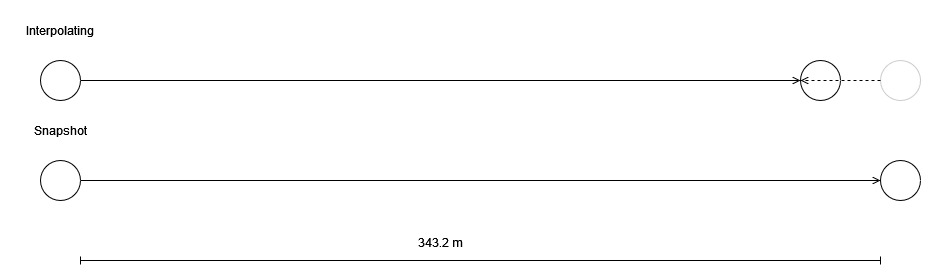
\includegraphics[width=\linewidth]{images/snapshot_explain.jpg}
    \caption{Difference between ray travelling distance using the newly developed interpolating method (top) as opposed to the snapshot method (bottom). In the interpolated version, the ray only travels part of the distance as the receiver travels the remainder.}
\end{figure}
The major downside of this snapshot approach is that it tends to introduce errors when objects or receivers move at high speeds.
As a simple example case, take the scene described in~\ref{SnapshotExplain}:
A receiver starts 343 meters away from an emitter and moves towards it at 1/9th the speed of sound, roughly 38 meters per second
(137.2 kilometers per hour, a speed most modern cars can reach without problems).
\newline
Using the snapshot approach, a ray traveling directly from emitter to receiver would arrive after travelling the full 343 meters,
taking 1 second for it to arrive at the receiver.
In actuality, in the time the ray takes to travel the first 90\% of that distance,
the receiver has already travelled the remaining 10\%, making for a response time of 0.9 seconds rather than 1 second.
\newline
While Bilibashi et al.~\cite{BVD20} have attempted to solve this issue,
they only aimed to simulate waves bouncing between a few set points, namely cars,
rather than simulating full room acoustics.
Their vector-based approach cannot be used for a full scene simulation.
\newline
To accurately simulate both edge cases occurring in the real world (such as the example above)
and hypothetical situations such as the test cases described below,
a new method needs to be developed.

\section{Scope}

This thesis proposes a method to simulate rays bouncing through arbitrary scenes with moving receivers and/or objects,
assuming all movement within the scene is known at time of calculation.
An improved way of checking for intersections between rays and objects is developed, accommodating for this new requirement.
Optimisations are evaluated and a time-based chunking method is developed to avoid needless intersection checks.
Additionally, a method is developed to to losslessly and efficiently store the multiple impulse responses created by re-calculating
the impulse responses for different points in time.
The goal of this research is to simulate effects such as the situation described in~\ref{SnapshotExplain} without errors introduced by the snapshot method
as well as recreate the acoustics of a hypothetical, rapidly rotating room.
Three test cases are developed for this and compared to an implementation of the snapshot method:
An empty scene with the sound receiver approaching the sound emitter at 1/9th the speed of sound,
a square room rapidly rotating
and a large, L-shaped room also rapidly rotating around one of its ends, with the receiver and emitter both sitting in said end.
\newline
Not within the scope of this thesis is a fully accurate simulation
including effects such as the differing bouncing behaviour sound waves show at different frequencies.
Only a proof of concept that shows that the idea of this new simulation method works is developed.
\newline
Side effects of moving scenes, such as sounds emitted by moving objects, are also discarded as they are irrelevant to
the changed intersection logic.
A note-worthy side effect that gets ignored is mass inertia:
The example case where this would become relevant is the inside of a linearly moving enclosed room, such as a driving car.
Due to mass inertia, sound waves travelling inside this moving rome behave the same as if the car stood still.
Since this effect is only relevant in a niche scenario and it can be simulated using a method that ignores movement entirely,
it can be ignored for this research.
\newline
Real-time applications cannot use this proposed method as it requires knowledge of objects' future movements ahead of time.
Further research is required to develop an alternative method for real-time or dynamic simulations.
A real-time approach could work by not calculating the rays' entire movements at emission time,
but instead keeping track of all moving rays and incrementally continuing their journey through the now updated scene
at recurring intervals.
